\section{Event reconstruction algorithms and performance}
\label{sec:larsoftreco}

The interpretation of the data from liquid-argon TPC detectors has
proven challenging, largely due to the wealth of information provided
in each event by the detector, but also due to the high rate of
multiple scattering and particle interactions, as well as the
projection of three-dimensional information onto a discretized
two-dimensional space of readout ADC counts on wires as functions of
time.  The flexibility of the {\it{art}}/LArSoft framework allows
multiple approaches to reconstructing and analyzing the data to be
explored, and different approaches taken depending on the targeted
physics deliverable.

The first step in processing the data is to uncompress it and read it
in to data structures that match the offline representation.  Because
the simulation steps historically preceded the DAQ formats, and
because the offline processing must flexibly accommodate changing DAQ
formats without rewriting the downstream processing software, the
choice is made to represent the data in the offline format.

\fixme{some duplication with the text below is still here. Need to merge
descriptions. But the reco steps really do diverge in the alternate methods}

Noise filtering is then applied.  Existing LArTPC experiments have a
large component of their noise from coherent sources -- sources that
affect many neighboring wires and/or neighboring readout channels
(channels from different planes may be interleaved in the front-end
electronics) together.  The data from these channels can then be used
to estimate what the noise is on any one of them, and then used to
subtract as much of the correlated noise component as possible.  A
drawback of this procedure is that signals also arrive on neighboring
channels at the same time, and this procedure reduces the signal as
well as the noise, in a manner that depends on the angle of a track or
shower with respect to the drift field.  Procedures that first
identify signal hits and protect them from
distortion~\cite{microboone_noise} are under study.

The raw signals are then processed through a signal deconvolution and
noise filtering step.  This step is done using a discrete Fourier
transform, the application of the deconvolution kernel and filter
function in frequency space, and then followed by an inverse discrete
Fourier transform.  The deconvolution kernel serves to convert the
bipolar induction-plane signals into unipolar estimates of the charge
arrival time, and serves to remove as much of the electronics
distortions from both the induction-plane signals and the
collection-plane signals as possible.  It is needed since the positive
lobe of the induction-plane signal from one charge deposit may cancel
the negative lobe of the signal from another charge deposit.  The
filter is a Wiener filter, where the expected signals and backgrounds
are obtained from data samples.  A typical band in which signal
frequencies lie is 10 KHz, while easily-filtered noise is at much
higher and lower frequencies.  A typical filter function is shown in
Figure~\ref{fig:wienerfilter}

\begin{figure}[htb]
\centering
%\includegraphics[width=0.95\textwidth]{figures/wienerfilter.png}
Include figure of the Wiener filter
\caption{The noise filter function applied to 35-ton data.  A similar
  procedure will produce a noise filter function for ProtoDUNE-SP}
\label{fig:wienerfilter}
\end{figure}

Hits are then identified by seeking deconvoluted signals exceeding
thresholds that are adjusted to minimize the creation of false noise
hits while preserving the true signal hits.  The standard LArSoft hit
finder fits Gaussians to the deconvoluted signals, and saves the
times, widths, and amplitudes of the Gaussians, as well as the sum of
the ADC readings in the time windows corresponding to the hits, as a
Gaussian function is not always representative of the charge arrival
distributin and the resolution of the calorimetry is improved by
summing the ADC counts.  The hits are associated with DAQ channels and
not wire segments, since, due to the wrapping of the induction-plane
wires in the ProtoDUNE-SP APA's, there is ambiguity of where the
charge contributing to the hit was deposited.  Because the wire angle
is chosen so that each induction wire intersects each collection-plane
wire at most one time, only two views are needed in order to identify
hits and resolve ambiguities.  A separate LArSoft module compares the
hits in the collection and induction views and assigns choices to
remove ambiguity, allowing reconstruction algorithms developed for
detectors without wrapped wires to be run with minimal modification.

Several approaches are then possible once hits are identified on wire
segments.  Two-dimensional reconstruction identifies tracks and
clusters in each view separately, and three-dimensional hypotheses for
the event are constructed by comparing the two-dimensional clusters'
images in the separate planes.  The clustering algorithm currently in
use is the Blurred Clustering Algorithm~\cite{blurredclustering}.  The
EMShower package~\cite{emshowerpackage} takes blurred clusters and
produces energies, angles, and start positions for the showers, as
well as the $dE/dx$ in the initial part of the shower.  Identifying
events with two showers consistent with $\pi^0\rightarrow\gamma\gamma$
decays allows for an {\it in situ} calibration of the electromagnetic
energy scale as well as the performance of shower identification and
reconstruction for photons that are produced inside the detector.  A
distribution of reconstructed $\pi^0$ masses in Monte Carlo is shown
in Figure~\ref{fig:pizeromass}.

\begin{figure}[htb]
\centering
%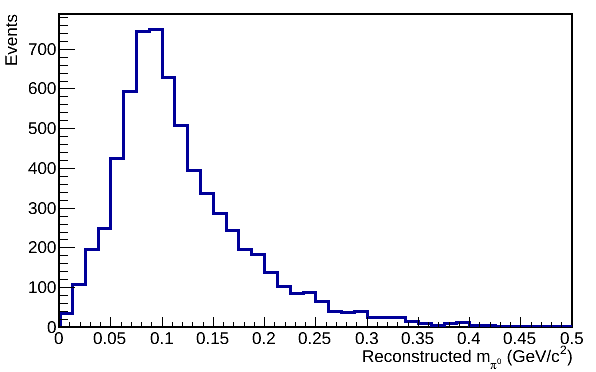
\includegraphics[width=0.95\textwidth]{figures/pizeromass.png}
Include pizero mass peak plot
\caption{The reconstructed invariant masses of $\pi^0$ candidates in
  Monte Carlo using the BlurredCluster and EMShower algorithms.  }
\label{fig:muonpandoraperf}
\end{figure}

The reconstruction framework PANDORA~\cite{pandora} also works by
building up a three-dimensional picture from two-dimensional
reconstructed objects.  PANDORA is a flexible framework developed for
ILC detector simulation, and provides a convenient way to develop
algorithms for reconstructing particles.  In all, more than 80
algorithms, each targeting a specific topology, have been incorporated
into PANDORA to date.  Multiple passes through reconstructing the data
are possible.  Different criteria for clustering hits into tracks and
showers may be applied when seeking cosmic rays for removal than for
identifying signal events.  PANDORA proceeds by clustering hits in 2D,
reconstructing vertices in 3D, reconstructing tracks in 3D,
reconstructing showers in 3D, a mop-up step in 2D and 3D, followed by
full event building in 3D.

The performance metrics are efficiency, purity, and completeness.  The
efficiency of the algorithm is the fraction of true particles that
match reconstructed objects within the bounds of pre-specified
criteria, such as matching position and length and the type of object
expected.  The purity of the reconstructed object is the fraction of
hits (or charge) included in that object that truly came from the
matched particle divided by the total number of hits (or charge)
included in the reconstructed cluster.  The completeness is defined as
the number of true hits that are found in a cluster or track or shower
expressed as a fraction of total true hits in that object.  Plots of
the efficiency and completeness for muons in charged-current $\nu_mu$
events in MicroBooNE are shown in Figure~\ref{fig:muonpandoraperf}.
The resolution of vertex-finding is shown in
Figure~\ref{fig:pandoraresolution}.

\begin{figure}[htb]
\centering
%\includegraphics[width=0.95\textwidth]{figures/muonpandoraperf.png}
Include figure of PANDORA performance for muons.  Efficiency and
completeness (purity too if we can get the plot).
\caption{The performance of PANDORA for muons in charged-current
  $\nu_mu$ events in MicroBooNE.  }
\label{fig:muonpandoraperf}
\end{figure}

A very successful approach to reconstruction is called the Projection
Matching Algorithm (PMA)~\cite{pma_algorithm}.  Instead of building up
a 3D hypothesis from 2D clusters, it instead starts with the 3D
hypothesis and compares the predicted data with the observed data.
PMA can take as input the output from different pattern recognition
algorithms, from BlurredCluster to WireCell (described below).  PMA
has successfully been used to reconstruct simulated beam particles in
ProtoDUNE-SP.  The spatial resolution of the particle entry point is
shown in Figure~\ref{PMAentryresolution}, the direction resolution in
Figure~\ref{fig:PMAdirection}, and the spatial resolution of the the
inelastic interaction point of charged pions in ProtoDUNE-SP is shown
in Figure~\ref{fig:PMApioninteraction}.

\begin{figure}[htb]
\centering
%\includegraphics[width=0.95\textwidth]{figures/PMAentryresolution.png}
Include figure of PMA's resolution on the entry point for charged
particles See Robert's talk from the April collab meeting
\caption{Spatial resolution on the 3D entry position of the primary
  charged particle from the beam in ProtoDUNE-SP, using the PMA
  reconstruction algorithm.}
\label{fig:PMAentryresolution}
\end{figure}

\begin{figure}[htb]
\centering
%\includegraphics[width=0.95\textwidth]{figures/PMAdirection.png}
Include figure of PMA's resolution on the direction for charged
particles See Robert's talk from the April collab meeting
\caption{Angular resolution of the momentum vector of the the primary
  charged particle from the beam in ProtoDUNE-SP, using the PMA
  reconstruction algorithm.}
\label{fig:PMAdirection}
\end{figure}

\begin{figure}[htb]
\centering
%\includegraphics[width=0.95\textwidth]{figures/PMApioninteraction.png}
Include figure of PMA's pion interaction position resolution.  See
Robert's talk from the April collab meeting
\caption{Vertex position resolution in $x$, $y$, and $z$ for the
  inelastic interaction of charged pions on liquid argon nuclei in
  ProtoDUNE-SP, using the PMA algorithm.}
\label{fig:PMApioninteraction}
\end{figure}
